\begin{figure}
	\centering
	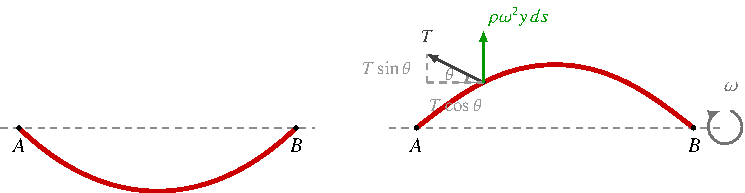
\includegraphics[width=\textwidth]{papers/elliptisch/images/troposkein.pdf}
	\caption{Links die hängende Schnur zwischen $A$ und $B$, die
	Kettenlinie $y(x) = a\cosh(x/a)$.
	Rechts dieselbe Schnur rotierend um die Achse $AB$, das
	Troposkein $y(x) = a\operatorname{sn}(x/c, k)$, mit der
	Zentrifugalkraft $\rho\omega^2y\,ds$ und der Seilspannung $T$ an
	einem Element bei Winkel $\theta$.}
	\label{fig:elliptisch:troposkein}
\end{figure}
